
%% bare_jrnl_compsoc.tex
%% V1.4b
%% 2015/08/26
%% by Michael Shell
%% See:
%% http://www.michaelshell.org/
%% for current contact information.
%%
%% This is a skeleton file demonstrating the use of IEEEtran.cls
%% (requires IEEEtran.cls version 1.8b or later) with an IEEE
%% Computer Society journal paper.
%%
%% Support sites:
%% http://www.michaelshell.org/tex/ieeetran/
%% http://www.ctan.org/pkg/ieeetran
%% and
%% http://www.ieee.org/ 
% The testflow support page is at:
% http://www.michaelshell.org/tex/testflow/
\documentclass[10pt,journal,compsoc]{IEEEtran}

\usepackage{graphicx}
%\graphicspath{{./BIBM/}}
%
% If IEEEtran.cls has not been installed into the LaTeX system files,
% manually specify the path to it like:
% \documentclass[10pt,journal,compsoc]{../sty/IEEEtran}
\ifCLASSOPTIONcompsoc
  % IEEE Computer Society needs nocompress option
  % requires cite.sty v4.0 or later (November 2003)
  \usepackage[nocompress]{cite}
\else
  % normal IEEE
  \usepackage{cite}
\fi
% *** GRAPHICS RELATED PACKAGES ***
%
\ifCLASSINFOpdf
  % \usepackage[pdftex]{graphicx}
  % declare the path(s) where your graphic files are
  % \graphicspath{{../pdf/}{../jpeg/}}
  % and their extensions so you won't have to specify these with
  % every instance of \includegraphics
  % \DeclareGraphicsExtensions{.pdf,.jpeg,.png}
\else
  % or other class option (dvipsone, dvipdf, if not using dvips). graphicx
  % will default to the driver specified in the system graphics.cfg if no
  % driver is specified.
  % \usepackage[dvips]{graphicx}
  % declare the path(s) where your graphic files are
  % \graphicspath{{../eps/}}
  % and their extensions so you won't have to specify these with
  % every instance of \includegraphics
  % \DeclareGraphicsExtensions{.eps}
\fi
% graphicx was written by David Carlisle and Sebastian Rahtz. It is
% required if you want graphics, photos, etc. graphicx.sty is already
% installed on most LaTeX systems. The latest version and documentation
% can be obtained at: 
% http://www.ctan.org/pkg/graphicx
% Another good source of documentation is "Using Imported Graphics in
% LaTeX2e" by Keith Reckdahl which can be found at:
% http://www.ctan.org/pkg/epslatex
%
% latex, and pdflatex in dvi mode, support graphics in encapsulated
% postscript (.eps) format. pdflatex in pdf mode supports graphics
% in .pdf, .jpeg, .png and .mps (metapost) formats. Users should ensure
% that all non-photo figures use a vector format (.eps, .pdf, .mps) and
% not a bitmapped formats (.jpeg, .png). The IEEE frowns on bitmapped formats
% which can result in "jaggedy"/blurry rendering of lines and letters as
% well as large increases in file sizes.
%
% You can find documentation about the pdfTeX application at:
% http://www.tug.org/applications/pdftex






% *** MATH PACKAGES ***
%
%\usepackage{amsmath}
% A popular package from the American Mathematical Society that provides
% many useful and powerful commands for dealing with mathematics.
%
% Note that the amsmath package sets \interdisplaylinepenalty to 10000
% thus preventing page breaks from occurring within multiline equations. Use:
%\interdisplaylinepenalty=2500
% after loading amsmath to restore such page breaks as IEEEtran.cls normally
% does. amsmath.sty is already installed on most LaTeX systems. The latest
% version and documentation can be obtained at:
% http://www.ctan.org/pkg/amsmath





% *** SPECIALIZED LIST PACKAGES ***
%
%\usepackage{algorithmic}
% algorithmic.sty was written by Peter Williams and Rogerio Brito.
% This package provides an algorithmic environment fo describing algorithms.
% You can use the algorithmic environment in-text or within a figure
% environment to provide for a floating algorithm. Do NOT use the algorithm
% floating environment provided by algorithm.sty (by the same authors) or
% algorithm2e.sty (by Christophe Fiorio) as the IEEE does not use dedicated
% algorithm float types and packages that provide these will not provide
% correct IEEE style captions. The latest version and documentation of
% algorithmic.sty can be obtained at:
% http://www.ctan.org/pkg/algorithms
% Also of interest may be the (relatively newer and more customizable)
% algorithmicx.sty package by Szasz Janos:
% http://www.ctan.org/pkg/algorithmicx




% *** ALIGNMENT PACKAGES ***
%
%\usepackage{array}
% Frank Mittelbach's and David Carlisle's array.sty patches and improves
% the standard LaTeX2e array and tabular environments to provide better
% appearance and additional user controls. As the default LaTeX2e table
% generation code is lacking to the point of almost being broken with
% respect to the quality of the end results, all users are strongly
% advised to use an enhanced (at the very least that provided by array.sty)
% set of table tools. array.sty is already installed on most systems. The
% latest version and documentation can be obtained at:
% http://www.ctan.org/pkg/array


% IEEEtran contains the IEEEeqnarray family of commands that can be used to
% generate multiline equations as well as matrices, tables, etc., of high
% quality.




% *** SUBFIGURE PACKAGES ***
%\ifCLASSOPTIONcompsoc
%  \usepackage[caption=false,font=footnotesize,labelfont=sf,textfont=sf]{subfig}
%\else
%  \usepackage[caption=false,font=footnotesize]{subfig}
%\fi
% subfig.sty, written by Steven Douglas Cochran, is the modern replacement
% for subfigure.sty, the latter of which is no longer maintained and is
% incompatible with some LaTeX packages including fixltx2e. However,
% subfig.sty requires and automatically loads Axel Sommerfeldt's caption.sty
% which will override IEEEtran.cls' handling of captions and this will result
% in non-IEEE style figure/table captions. To prevent this problem, be sure
% and invoke subfig.sty's "caption=false" package option (available since
% subfig.sty version 1.3, 2005/06/28) as this is will preserve IEEEtran.cls
% handling of captions.
% Note that the Computer Society format requires a sans serif font rather
% than the serif font used in traditional IEEE formatting and thus the need
% to invoke different subfig.sty package options depending on whether
% compsoc mode has been enabled.
%
% The latest version and documentation of subfig.sty can be obtained at:
% http://www.ctan.org/pkg/subfig




% *** FLOAT PACKAGES ***
%
%\usepackage{fixltx2e}
% fixltx2e, the successor to the earlier fix2col.sty, was written by
% Frank Mittelbach and David Carlisle. This package corrects a few problems
% in the LaTeX2e kernel, the most notable of which is that in current
% LaTeX2e releases, the ordering of single and double column floats is not
% guaranteed to be preserved. Thus, an unpatched LaTeX2e can allow a
% single column figure to be placed prior to an earlier double column
% figure.
% Be aware that LaTeX2e kernels dated 2015 and later have fixltx2e.sty's
% corrections already built into the system in which case a warning will
% be issued if an attempt is made to load fixltx2e.sty as it is no longer
% needed.
% The latest version and documentation can be found at:
% http://www.ctan.org/pkg/fixltx2e


%\usepackage{stfloats}
% stfloats.sty was written by Sigitas Tolusis. This package gives LaTeX2e
% the ability to do double column floats at the bottom of the page as well
% as the top. (e.g., "\begin{figure*}[!b]" is not normally possible in
% LaTeX2e). It also provides a command:
%\fnbelowfloat
% to enable the placement of footnotes below bottom floats (the standard
% LaTeX2e kernel puts them above bottom floats). This is an invasive package
% which rewrites many portions of the LaTeX2e float routines. It may not work
% with other packages that modify the LaTeX2e float routines. The latest
% version and documentation can be obtained at:
% http://www.ctan.org/pkg/stfloats
% Do not use the stfloats baselinefloat ability as the IEEE does not allow
% \baselineskip to stretch. Authors submitting work to the IEEE should note
% that the IEEE rarely uses double column equations and that authors should try
% to avoid such use. Do not be tempted to use the cuted.sty or midfloat.sty
% packages (also by Sigitas Tolusis) as the IEEE does not format its papers in
% such ways.
% Do not attempt to use stfloats with fixltx2e as they are incompatible.
% Instead, use Morten Hogholm'a dblfloatfix which combines the features
% of both fixltx2e and stfloats:
%
% \usepackage{dblfloatfix}
% The latest version can be found at:
% http://www.ctan.org/pkg/dblfloatfix




%\ifCLASSOPTIONcaptionsoff
%  \usepackage[nomarkers]{endfloat}
% \let\MYoriglatexcaption\caption
% \renewcommand{\caption}[2][\relax]{\MYoriglatexcaption[#2]{#2}}
%\fi
% endfloat.sty was written by James Darrell McCauley, Jeff Goldberg and 
% Axel Sommerfeldt. This package may be useful when used in conjunction with 
% IEEEtran.cls'  captionsoff option. Some IEEE journals/societies require that
% submissions have lists of figures/tables at the end of the paper and that
% figures/tables without any captions are placed on a page by themselves at
% the end of the document. If needed, the draftcls IEEEtran class option or
% \CLASSINPUTbaselinestretch interface can be used to increase the line
% spacing as well. Be sure and use the nomarkers option of endfloat to
% prevent endfloat from "marking" where the figures would have been placed
% in the text. The two hack lines of code above are a slight modification of
% that suggested by in the endfloat docs (section 8.4.1) to ensure that
% the full captions always appear in the list of figures/tables - even if
% the user used the short optional argument of \caption[]{}.
% IEEE papers do not typically make use of \caption[]'s optional argument,
% so this should not be an issue. A similar trick can be used to disable
% captions of packages such as subfig.sty that lack options to turn off
% the subcaptions:
% For subfig.sty:
% \let\MYorigsubfloat\subfloat
% \renewcommand{\subfloat}[2][\relax]{\MYorigsubfloat[]{#2}}
% However, the above trick will not work if both optional arguments of
% the \subfloat command are used. Furthermore, there needs to be a
% description of each subfigure *somewhere* and endfloat does not add
% subfigure captions to its list of figures. Thus, the best approach is to
% avoid the use of subfigure captions (many IEEE journals avoid them anyway)
% and instead reference/explain all the subfigures within the main caption.
% The latest version of endfloat.sty and its documentation can obtained at:
% http://www.ctan.org/pkg/endfloat
%
% The IEEEtran \ifCLASSOPTIONcaptionsoff conditional can also be used
% later in the document, say, to conditionally put the References on a 
% page by themselves.




% *** PDF, URL AND HYPERLINK PACKAGES ***
%
%\usepackage{url}
% url.sty was written by Donald Arseneau. It provides better support for
% handling and breaking URLs. url.sty is already installed on most LaTeX
% systems. The latest version and documentation can be obtained at:
% http://www.ctan.org/pkg/url
% Basically, \url{my_url_here}.





% *** Do not adjust lengths that control margins, column widths, etc. ***
% *** Do not use packages that alter fonts (such as pslatex).         ***
% There should be no need to do such things with IEEEtran.cls V1.6 and later.
% (Unless specifically asked to do so by the journal or conference you plan
% to submit to, of course. )


% correct bad hyphenation here
\hyphenation{op-tical net-works semi-conduc-tor}


\begin{document}
%
% paper title
% Titles are generally capitalized except for words such as a, an, and, as,
% at, but, by, for, in, nor, of, on, or, the, to and up, which are usually
% not capitalized unless they are the first or last word of the title.
% Linebreaks \\ can be used within to get better formatting as desired.
% Do not put math or special symbols in the title.
\title{ScSpark: Low-Redundancy Disk Access and High-Performance Tool for the Single-Cell RNA Sequenceing Data Processing}
%
%
% author names and IEEE memberships
% note positions of commas and nonbreaking spaces ( ~ ) LaTeX will not break
% a structure at a ~ so this keeps an author's name from being broken across
% two lines.
% use \thanks{} to gain access to the first footnote area
% a separate \thanks must be used for each paragraph as LaTeX2e's \thanks
% was not built to handle multiple paragraphs
%
%
%\IEEEcompsocitemizethanks is a special \thanks that produces the bulleted
% lists the Computer Society journals use for "first footnote" author
% affiliations. Use \IEEEcompsocthanksitem which works much like \item
% for each affiliation group. When not in compsoc mode,
% \IEEEcompsocitemizethanks becomes like \thanks and
% \IEEEcompsocthanksitem becomes a line break with idention. This
% facilitates dual compilation, although admittedly the differences in the
% desired content of \author between the different types of papers makes a
% one-size-fits-all approach a daunting prospect. For instance, compsoc 
% journal papers have the author affiliations above the "Manuscript
% received ..."  text while in non-compsoc journals this is reversed. Sigh.

\author{Michael~Shell,~\IEEEmembership{Member,~IEEE,}
        John~Doe,~\IEEEmembership{Fellow,~OSA,}
        and~Jane~Doe,~\IEEEmembership{Life~Fellow,~IEEE}% <-this % stops a space
\IEEEcompsocitemizethanks{\IEEEcompsocthanksitem M. Shell was with the Department
of Electrical and Computer Engineering, Georgia Institute of Technology, Atlanta,
GA, 30332.\protect\\
% note need leading \protect in front of \\ to get a newline within \thanks as
% \\ is fragile and will error, could use \hfil\break instead.
E-mail: see http://www.michaelshell.org/contact.html
\IEEEcompsocthanksitem J. Doe and J. Doe are with Anonymous University.}% <-this % stops an unwanted space
\thanks{Manuscript received April 19, 2005; revised August 26, 2015.}}

% note the % following the last \IEEEmembership and also \thanks - 
% these prevent an unwanted space from occurring between the last author name
% and the end of the author line. i.e., if you had this:
% 
% \author{....lastname \thanks{...} \thanks{...} }
%                     ^------------^------------^----Do not want these spaces!
%
% a space would be appended to the last name and could cause every name on that
% line to be shifted left slightly. This is one of those "LaTeX things". For
% instance, "\textbf{A} \textbf{B}" will typeset as "A B" not "AB". To get
% "AB" then you have to do: "\textbf{A}\textbf{B}"
% \thanks is no different in this regard, so shield the last } of each \thanks
% that ends a line with a % and do not let a space in before the next \thanks.
% Spaces after \IEEEmembership other than the last one are OK (and needed) as
% you are supposed to have spaces between the names. For what it is worth,
% this is a minor point as most people would not even notice if the said evil
% space somehow managed to creep in.



% The paper headers
\markboth{Journal of \LaTeX\ Class Files,~Vol.~14, No.~8, August~2015}%
{Shell \MakeLowercase{\textit{et al.}}: Bare Demo of IEEEtran.cls for Computer Society Journals}
% The only time the second header will appear is for the odd numbered pages
% after the title page when using the twoside option.
% 
% *** Note that you probably will NOT want to include the author's ***
% *** name in the headers of peer review papers.                   ***
% You can use \ifCLASSOPTIONpeerreview for conditional compilation here if
% you desire.



% The publisher's ID mark at the bottom of the page is less important with
% Computer Society journal papers as those publications place the marks
% outside of the main text columns and, therefore, unlike regular IEEE
% journals, the available text space is not reduced by their presence.
% If you want to put a publisher's ID mark on the page you can do it like
% this:
%\IEEEpubid{0000--0000/00\$00.00~\copyright~2015 IEEE}
% or like this to get the Computer Society new two part style.
%\IEEEpubid{\makebox[\columnwidth]{\hfill 0000--0000/00/\$00.00~\copyright~2015 IEEE}%
%\hspace{\columnsep}\makebox[\columnwidth]{Published by the IEEE Computer Society\hfill}}
% Remember, if you use this you must call \IEEEpubidadjcol in the second
% column for its text to clear the IEEEpubid mark (Computer Society jorunal
% papers don't need this extra clearance.)



% use for special paper notices
%\IEEEspecialpapernotice{(Invited Paper)}



% for Computer Society papers, we must declare the abstract and index terms
% PRIOR to the title within the \IEEEtitleabstractindextext IEEEtran
% command as these need to go into the title area created by \maketitle.
% As a general rule, do not put math, special symbols or citations
% in the abstract or keywords.
\IEEEtitleabstractindextext{%
\begin{abstract}
High-throughput single-cell RNA sequencing (scRNA-seq) data processing pipelines typically integrate multiple modules to transform raw scRNA-seq data to gene expression matrices, including barcode processing, sequence quality control, genome alignment and transcript counting. 
With the drastic increase in scRNA-seq data size, file input/output (IO) has become a bottleneck of the processing speed of available tools. 
In this study, we took advantage of Apache Spark's in-memory computing and inherent scalability to develop a new Java-based scRNA-seq data processing pipeline, named scSpark. 
%We combined Spark and our proposed functionalities to implement sequence quality control and transcript counting. 
To reduce unneccessary disk access while reading FASTQ files and writing SAM files, we used Java Native Interface (JNI) to deliver FASTQ Resilient Distributed Datasets (RDD), and then retrieved genome mapping results to SAM RDD. 
By allocating scRNA-seq data and processing tasks to computer cluster, the scSpark toolkit can significantly reduce disk access for saving and loading temporary results. 
To test the performance of scSpark, we built a spark cluster on Aliyun, and evaluated its computational performance and biological analysis robustness with several state-of-the-art data processing pipelines. The results indicate that scSpark is more efficient and more scalable than any available tool. 
\end{abstract}

% Note that keywords are not normally used for peerreview papers.
\begin{IEEEkeywords}
Intermediate Data, Fast, Scalable.
\end{IEEEkeywords}}


% make the title area
\maketitle


% To allow for easy dual compilation without having to reenter the
% abstract/keywords data, the \IEEEtitleabstractindextext text will
% not be used in maketitle, but will appear (i.e., to be "transported")
% here as \IEEEdisplaynontitleabstractindextext when the compsoc 
% or transmag modes are not selected <OR> if conference mode is selected 
% - because all conference papers position the abstract like regular
% papers do.
\IEEEdisplaynontitleabstractindextext
% \IEEEdisplaynontitleabstractindextext has no effect when using
% compsoc or transmag under a non-conference mode.



% For peer review papers, you can put extra information on the cover
% page as needed:
% \ifCLASSOPTIONpeerreview
% \begin{center} \bfseries EDICS Category: 3-BBND \end{center}
% \fi
%
% For peerreview papers, this IEEEtran command inserts a page break and
% creates the second title. It will be ignored for other modes.
\IEEEpeerreviewmaketitle



\IEEEraisesectionheading{\section{Introduction}\label{sec:introduction}}
% The very first letter is a 2 line initial drop letter followed
% by the rest of the first word in caps (small caps for compsoc).
% 
% form to use if the first word consists of a single letter:
% \IEEEPARstart{A}{demo} file is ....
% 
% form to use if you need the single drop letter followed by
% normal text (unknown if ever used by the IEEE):
% \IEEEPARstart{A}{}demo file is ....
% 
% Some journals put the first two words in caps:
% \IEEEPARstart{T}{his demo} file is ....
% 
% Here we have the typical use of a "T" for an initial drop letter
% and "HIS" in caps to complete the first word.


%------Introduciton
% Individual cells are the smallest unit of life, such as tissues and organs.
% According to the central dogma of molecular biology, one of the major factors that determines the function of every cell is its transcriptional program.
% In the era of precision medicine, scientific experiments to explore the function of each cell have become crucial. 
\IEEEPARstart{S}{ingle} cell is the fundamental unit of a living organism. In the era of precision medicine, exploring the gene expression at single cell level has become crucial. In the past decade, RNA-seq has been widely used to study gene expression patterns in large-scale biological samples. However, the resolution of bulk RNA-seq could only reach the average level of cell populations. Single-cell RNA sequencing(scRNA-seq) essentially reveals the transcriptional status at single cell level, which provides the basis for subsequent bioinformatics analysis~\cite{Papalexi2018SinglecellRS}. 

High-throughput(HT) scRNA-seq protocols, which enable transcript sequencing of thousands of cells simultaneously in a single experiment, have emerged as powerful tools to identify and characterize cell types in complex and heterogeneous tissues~\cite{Zhang2019ComparativeAO}.
% are the most popular strategies currently for scRNA-seq technology~\cite{Zhang2019ComparativeAO}. 
Among them, Drop-seq~\cite{Macosko2015HighlyPG}, inDrop~\cite{Klein2015DropletBF} and 10X\cite{Zheng2017Massively} are the three most widely used protocols. 
Two important barcodes, named cell barcode (CB) and unique molecular identifier (UMI) are introduced in scRNA-seq~\cite{Rosenberg2018SinglecellPO}~\cite{Cao2017ComprehensiveSC}. 
CB, which assigns different sequences to each cell for transcriptional source retrieval after sequencing, greatly increases the total length of sequence and reduces the cost of scRNA-seq~\cite{Macosko2015HighlyPG}~\cite{Klein2015DropletBF}. 
These barcodes allow reads to be demultiplexed after the cells have been assembled for sequencing~\cite{Tian2018scPipe}.
In addition to cell barcodes, UMIs are random oligonucleotide barcodes that are used in scRNA-seq experiments~\cite{Kivioja2012Counting}~\cite{Camara2017Methods}.
By UMI, we could distinguish the same copies located in different molecules from those in the same molecule for PCR amplification ~\cite{Smith2017UMItools}.

In the scRNA-seq experiment, the use of multi-level barcodes presented additional challenges for data processing, which was quite different from traditional bulk RNA-seq and low-throughput scRNA-seq experiments. 
In recent years, researchers have developed multiple scRNA-seq data processing tools, typically implementing steps including sequence quality control, genome alignment, and transcript counting to convert raw scRNA-seq data into a gene expression matrix for further downstream analysis. 
The first step is filtering FASTQ readings with low quality CB based on user-defined thresholds. 
This step eliminates most of the false CBs, greatly improving the accuracy of the CBs that need to be considered for counting and reducing the number of CBs. 
The remaining FASTQ reads will map to genomes using the splice-aware aligner, such as STAR~\cite{Dobin2013STAR} or HISAT2~\cite{Kim2015HISAT}. 
Among them, STAR is the most widely used. A number of popular scRNA-seq data processing tools use STAR for mapping, such as UMI-Tools, CellRanger, zumis, scPipe, and STARsolo. 
Previous baseline studies have shown that STAR is one of the most reliable reference genomic aligner for RNA-Seq analysis~\cite{Baruzzo2017SimulationbasedCB}. 
Next, reads are assigned to genes and count matrices for UMIs are generated.~\cite{Parekh2018zUMIs}. 

Nowadays, there are many tools to preprocess scRNA-seq, among which the most popular is CellRanger~\cite{Zheng2017Massively}, UMI-tools~\cite{Smith2017UMItools} and STARsolo~\cite{Blibaum2019STARsolo}. 
CellRanger is a highly integrated data process software tailored by 10X Genomics for single-cell RNA sequencing analysis and it performs comparatively well on machine with enough CPU and memory resources in the big data set, but did badly in small data set. CellRanger performs best under large data sets among existing tools~\cite{Gao2020Comparison}.
UMI-tools~\cite{ref_url1} is an open source tool with an impressively clear process.
STARsolo~\cite{Blibaum2019STARsolo} has improved the parallelism of sequence mapping and counting procedures, and achieved good performance on a single machine.
It is a pity that all avaliable tools only run on a single machine with slow running speed, and cannot be extended to multiple nodes.

There have been many studies using big data framework like Hadoop~\cite{ref_url2} and Spark~\cite{ref_url3} to optimize Next Generation Sequencing (NGS) Data Processing. 
Due to more efficiency in utilizing memory computing, Spark is a better big data computing framework than Hadoop's MapReduce~\cite{Dean2008MapReduce, Zaharia2012Resilient}. 
SparkBWA~\cite{Abun2016SparkBWA} and GPF~\cite{Li2018Highperformance} are good frameworks with Spart for improving the efficiency of NGS data processing. 
Falco~\cite{Yang2017Falco} has tried to use Spark in scRNA-seq data preprocessing, but it has two limitations. 

Firstly, Falco can't deal with CBs and UMIs, so it is incompatible with any HT scRNA-seq protocol.
Secondly, Falco only uses Spark to simply concatenate the aligner and the feature quantitative softwares, which does not reduce the amount of disk reads and writes during alignment and transcript counting.
Falco’s operations have lots of redundancy disk access which causes its insufficient utilization of Spark’s in-memory computation well. 

The increase of scRNA-seq datasets require more efficient and faster data processing tools. However, the current scRNA-seq data preprocessing tools were designed without considering of the scalability, which could only run on a single computer and could not be extended to a cluster. From UMI-Tools and CellRanger to STARsolo, parallelism and performance has increased; However, due to the limit of a single machine, all of them have no scalability . 
The traditional single machine serial processing mode has been unable to meet the demand of computing and storage resources for super-large scale scRNA-seq data.
Different with Falco, we enhanced STAR's file I/O interface to reduce redundant disk access.
In the end, to achieve parallel and in-memory computing, scSpark implemented transcript counting by combining Spark function and our method that can distributed cumpute the result and generated by a graph algorithm.
Our work utilized Spark system architecture to develop a quick and scalable scRNA-seq data preprocessing tool. 

\section{Method}
\subsection{Overview}
We implemented sequence quality control, genome alignment, and transcript counting based on Spark framework. 
We run program across the cluster and default cache data in memory. 
Single machine's capacity is not sufficient to adapt the increasing scRNA-seq data size and the time to process intermediate files occupies a more significant proportion on total time. 
Therefore, reducing the disk access of intermediate files and improving the upstream data process's scalability is the main way to improve avaliable pipelines. 
ScSpark is based on UMI-tools.

\subsection{Spark Version Sequence Quality Control}
\begin{figure}
	\includegraphics[width=0.45\textwidth]{fig1.pdf}
	\caption{An overview of sequence quality control module based on Spark.} \label{fig1}
\end{figure}  
Large FASTQ files can be loaded in each node's memory parallel and the loading speed doesn't limit by single node disk access speed. 
As shown in Fig~\ref{fig1}, the sequence quality control step typically consists of two main components, i)generating a whitelist including identities of the true cell barcodes is unknown and ii)filtering FASTQ R1 with the whitelist and extracting FASTQ R2 according to filtered FASTQ R1's index.

We loaded each file splits of FASTQ R1 to memory, and abstract them as FASTQ R1 RDD. 
Then we calculated the number of occurences for each CB and selected the most frequent CBs, named whitelist RDD, as intermediate results. 
By using reduceByKey function, each barcode could be counted parallelly in each split of FASTQ R1 RDD and we coould merge each split's result in the end. 
After that we can use the result to generate whitelist RDD by Spark's sort and take function, both of which can parallelly compute in the cluster. 
The filtered FASTQ R1 RDD could be easily got by using the join function to find which read's cell barcode is in the whitelist RDD. 
And then we used filter function to extract FASTQ R2 RDD. 
The last step in sequence quality control was using join function again to combine filtered FASTQ R1 RDD and FASTQ R2 RDD with the same index. 
\subsection{Eleminate redundancy disk access in Aligner step}
\begin{figure}
	\includegraphics[width=0.45\textwidth]{fig2.pdf}
	\caption{New way to implement STAR's interface.} \label{fig2}
\end{figure}
Apart from Cellranger we can't know how it implements because it isn't an open source software. 
In previous pipeline, STAR needs to load extracted FASTQ R2 file or FASTQ R1 file. FASTQ R2 file and whitelist file will generate unneccessary disk access. 
We choose STAR as our aligner but avoid loading extracted FASTQ R2 and FASTQ R1 twice. 
As shown in Fig~\ref{fig2}, we utilized Java Native Interface to transfer extracted FASTQ R2 RDD's data to STAR program, and then run the STAR process.
The STAR aligner was encapsulated as a shared object and invoked the shared object as our aligner. 
To overcome imbalance problem of node's data volume, we repartitioned the extracted FASTQ R2 RDD, and then each node could run STAR parallelly with counterpoise data volume. 
We also found if node's in memory was enough, we could start up more than one STAR's in one node to achieve better parallel computing. 
The SAM or BAM file as STAR's output could generate more disk access waste than STAR's input. Here, we refered STAR-solo's solution to solve the problem by combining aligner and count. 
We used Java Native Interface again to transfer STAR results and directly abstract them to SAM RDD. 
This operation is parallel and totally in memory. 

\subsection{Count with multi-node}
\begin{figure}
	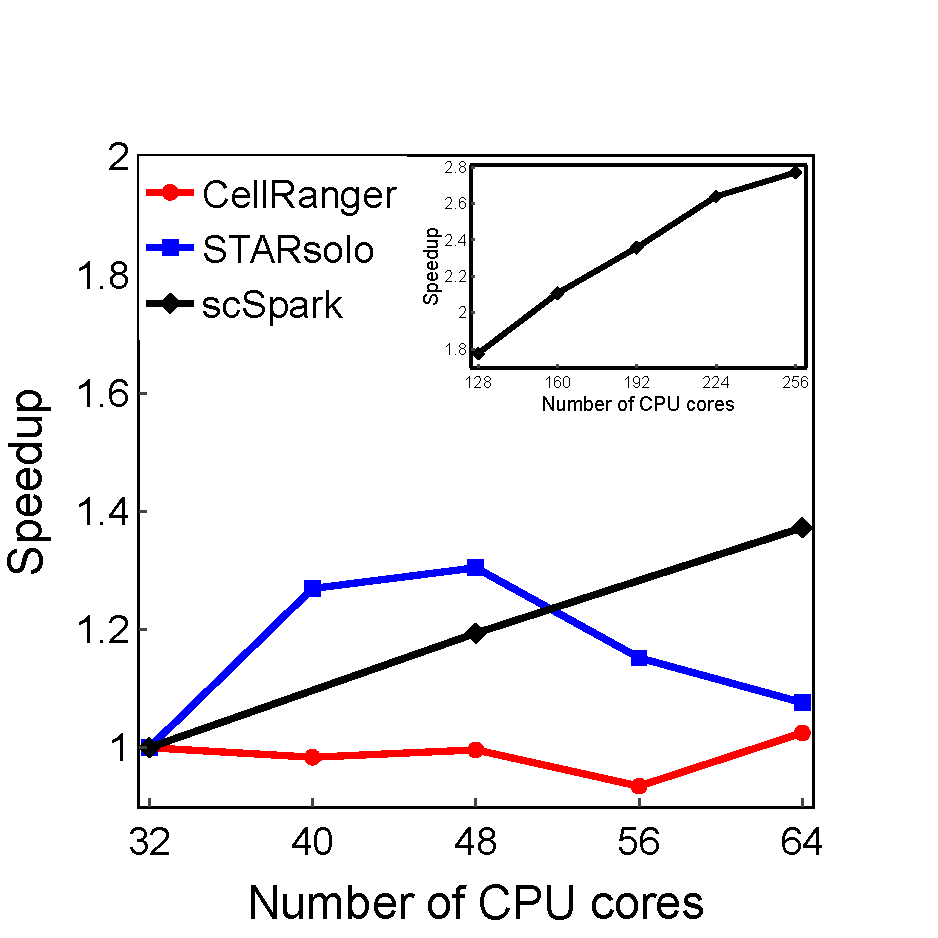
\includegraphics[width=0.45\textwidth]{fig3.pdf}
	\caption{An overview of Spark version count.} \label{fig3}
\end{figure}
As shown in Fig~\ref{fig3}, to take advantage of multi-node's compute capability, we used a new way to implement the count step. 
Except for SAM RDD that were generated in the previous step, we loaded GTF file to memory and abstract them as GTF RDD. 
Then we grouped SAM RDD and GTF RDD according to their cell name. 
Then we used flatMap function to parallelly compute each cell's read count. 
In the end, we collected results in all nodes, and the result files would produce the only output disk access in the whole program. 
ScSpark breaks the limitation of one node's computing and achieved large scalability. 

\section{Results}
We evaluated the speed and scalabilty for each step of scSpark to show the advantage of scSpark compared with the available pipelines. 
\subsection{Experiment environments and Data Sets prepare}
We used Apache Spark version 2.1.0 as our in-memory computing environment.
The Spark cluster consists of Aliyun's ECS, and each node consists of 16 vCPU.
(Intel Xeon(Cascade Lake) Platinum 8269CY at 2.5GHz), 128 GBytes of DRAM and 400 GBits ESSD.

An example scRNA-seq dataset generated by 10X Genomics on their platform was used in our experiments.
10X-PBMC-10k dataset: 10X Genomics v3 10k peripheral blood mononuclear cell (PBMC) from a healthy donor~\cite{ref_url4}.
It contains two gzipped FASTQ files. After unzipping, FASTQ R1's size is 69 Gbytes and FASTQ R2's size is 144 Gbytes. Each of the file contain 640 millions records.
We used STAR as our aligner, mapping to an index built on the human NCBI38 reference which called GRCh38.p12.genome.fa and use genome.gtf to filter the SAM~\cite{ref_url5}.
To evaluate the reason of why scSpark have a scalability ceiling and to experiment more convenient, we splitted FASTQ file to 100 millions, 160 millions and 320 millions records. 
\subsection{Efficiency Evaluation}
\begin{table}
	\centering
	\caption{previous pipeline and scSpark's performance comparisione}\label{tab1}
	\resizebox{0.45\textwidth}{!} {
	\begin{tabular}{l | l | l  l}
		\hline
		System &  Cores & Spend time(s) \\
		%\hline
		&  & 100M reads & 640M reads  \\
		\hline
		UMI-tools & 64 cores & 7254 & 44160 \\
		%\hline
		CellRanger & 64 cores & 6000 & 11700 \\
		%\hline
		STAR-solo & 64 cores &  5820 & 8100 \\
		%\hline
		scSpark & 4*16 cores & 354 & - \\
		& 8*16 cores & 210 & - \\
		& 16*16 cores & - & 841 \\
		\hline
	\end{tabular}
	}
\end{table}
Limited by single machine's CPU cores, we only took 64 cores in preivous pipeline test.
Table~\ref{tab1} shown a summary of all the pipelines's performance.
We could see scSpark's speed is much more quick than any available pipeline in the same CPU cores environment.
And scSpark could get improvement when the cluster's CPU cores number increased.
\begin{table}
	\centering
	\caption{Performance comparision for each step}\label{tab2}
	\resizebox{0.45\textwidth}{!} {
	\begin{tabular}{l | l | l | l | l}
		\hline
		System & Cores & filter & align & count \\
		\hline
		UMI-tools(100 million reads) & 64 cores & 9720 & 600 & 1740 \\
		%\hline
		UMI-tools(640 million reads) & 64 cores & 33600 & 2160 & 8400 \\
		%\hline
		scSpark(100 million reads) & 4*16 cores & 31 & 270 & 53 \\
		%\hline
		scSpark(640 million reads) & 16*16 cores & 81 & 447 & 313 \\
		\hline
	\end{tabular} }
\end{table}
Due to CellRanger isn't an open source software and STARsolo implements pipeline in a different way, we choose UMI-tools as scSpark each step's baseline.
As table~\ref{tab2} shown, scSpark is much faster than the previous pipeline in any single step.
We could see the most significant improvement came from the filtering step because we made a traditional single thread operation to parallelly computing in multi-machines and eliminates redundancy disk access.
For the same reason, scSpark's countting step also got considerable improvement.

\subsection{Scalability Evalution}
\begin{figure}
	\includegraphics[width=0.5\textwidth]{fig4.pdf}
	\caption{Pipeline Scalability.} \label{fig4}
\end{figure}
ScSpark's second advantage is that it could get near linear improvement when the cluster's CPU core number increased. 
To test the scalability, we used 16 CPU cores performance as previous pipeline's baseline and 64 CPU cores performance as scSpark's baseline. 
We used a small sample which had 100 millions records to compare speedup. 
As shown in Fig~\ref{fig5}, we found that when CPU cores number increased, our program could get near linear speedup. 
In addition, we found if the CPU cores number exceeds a ceiling, both previous pipeline and scSpark will speedup nearly stop. 
Umi-tools did not show any scalabiliy and even a little slow down when the CPU cores number increased. 
STARsolo and CellRanger shown a little improve when the CPU cores increased to 32 from 16, but quickly stopped speedup. 
These results show that scSpark's scalability has great improvement. 
\subsection{Comparsion each step performance's increase}
\begin{figure}
	\includegraphics[width=0.5\textwidth]{fig5.pdf}
	\caption{Each step consumes time.} \label{fig5}
\end{figure}
We also recorded each step's process time to know the reason of the improvement.
As shown in Fig~\ref{fig5}, we found our program's scalability mainly came from the alignment step, which consumed most time in the whole program.
Next, we counted how much records scSpark's STAR program can process.
We found that, as shown in Fig~\ref{fig6}, STAR's mapping speed was influenced by the data size and dataset with small size will lost its scalability earier than those with large size.
\begin{figure}
	\includegraphics[width=0.5\textwidth]{fig6.pdf}
	\caption{Invoked STAR's mapping step.} \label{fig6}
\end{figure}

\begin{table}
	\centering
	\caption{Processing speed w.r.t. data size}\label{tab3}
	\resizebox{0.45\textwidth}{!}
	{
	\begin{tabular}{l | l | l | l | l}
		\hline
		Volume(million reads) & 10 & 50 & 100 & 640 \\
		\hline
		Speed(million reads per hour) & 250.28 & 503.83 & 503.02 & 950 \\
		\hline
	\end{tabular}
	}
\end{table}

Then we tested STAR program, and found the mapping speed was also influenced by data size. 
As Table~\ref{tab3} shown, the speed of STAR mapping increased when the size of data increase. 
So when we got scalability by increasing partition, each partition's read number decreased and it would limit the scalability improvement

\subsection{Performance Analysis}
We tested performance to find the bottleneck of scSpark.
We used 640 millions records of FASTQ data to evaluate two aspects of scSpark.
First we compared network shuffle and disk access spend by scSpark and compute proportions of time, which helped to find whether network shuffle or disk access occupies too much time.
Secondy, we tested CPU and memory usage, to ensure which resources would cause scSpark's bottleneck.

\subsubsection{Network and Disk Behavior of scSpark}
\begin{figure}
	\includegraphics[width=0.5\textwidth]{fig7.pdf}
	\caption{Each step consumes time.} \label{fig7}
\end{figure}
We computed network time by summing up the time that our scSpark shuffle data in multi machine. 
Disk access comes from loading FASTQ, STAR's index and GTF files. 
The ideal situation is tasks did not waste any time in disk access and network shuffle. 
We found that scSpark's computing time occupied most execute time. 
Except STAR's index file, all files' disk access distributed to each node would improve whole system's loading speed. 
And we found the time that waste in shuffling doesn't occupy too much time. 

\subsubsection{CPU and Memory usage of scSpark}
\begin{figure}
	\includegraphics[width=0.5\textwidth]{fig8.pdf}
	\caption{CPU and Memory usage of scSpark.} \label{fig8}
\end{figure}
We monitored scSpark's CPU and memory usage during processing. 
As Fig~\ref{fig8} shown, in sequence quality control step, scSpark highly exploited each node's multi cores CPU to achieve speedup. 
Other pipelines' single thread solution's CPU usage is much lower than scSpark. 
We found that scSpark's boundary mainly came from genome alignment.
Because we invoked STAR as our alignment tool, and STAR's program naturally occupy most proportion of memory in this step.

\subsubsection{Biological verification}
ScSpark is developed based on UMI-tools, which has been fully verified in terms of accuracy. 
This section we used the gene expression matrix obtained by scSpark and UMI-tools to perform downstream analysis of scRNA-seq data. 
We compared transcript counting results and clusters of cells in the hgmm-1k-v3 dataset to verify the correlation between scSpark and UMI-tools. 

As Fig~\ref{fig9} shown, for each after processing cell barcode, their gene expression matrix approximate fit $y=x$, $R^{2}$ closed to 0.9998.
\begin{figure}
	\includegraphics[width=0.5\textwidth]{fig9.pdf}
	\caption{The correlation of transcript counting results for scSpark and UMI-tools.} \label{fig9}
\end{figure}
Furthermore, we used Seurat to obtain tSNE plots for the visualization of cell clusters. 
And as Fig~\ref{fig10} shown, tSNE cell clustering result showed high corrleation between ScSpark and UMI-tools.
\begin{figure}
	\includegraphics[width=0.5\textwidth]{fig10.pdf}
	\caption{tSNE plots based on scSpark and UMI-tools' gene expression matrices.} \label{fig10}
\end{figure}
% needed in second column of first page if using \IEEEpubid
%\IEEEpubidadjcol

% An example of a floating figure using the graphicx package.
% Note that \label must occur AFTER (or within) \caption.
% For figures, \caption should occur after the \includegraphics.
% Note that IEEEtran v1.7 and later has special internal code that
% is designed to preserve the operation of \label within \caption
% even when the captionsoff option is in effect. However, because
% of issues like this, it may be the safest practice to put all your
% \label just after \caption rather than within \caption{}.
%
% Reminder: the "draftcls" or "draftclsnofoot", not "draft", class
% option should be used if it is desired that the figures are to be
% displayed while in draft mode.
%
%\begin{figure}[!t]
%\centering
%\includegraphics[width=2.5in]{myfigure}
% where an .eps filename suffix will be assumed under latex, 
% and a .pdf suffix will be assumed for pdflatex; or what has been declared
% via \DeclareGraphicsExtensions.
%\caption{Simulation results for the network.}
%\label{fig_sim}
%\end{figure}

% Note that the IEEE typically puts floats only at the top, even when this
% results in a large percentage of a column being occupied by floats.
% However, the Computer Society has been known to put floats at the bottom.


% An example of a double column floating figure using two subfigures.
% (The subfig.sty package must be loaded for this to work.)
% The subfigure \label commands are set within each subfloat command,
% and the \label for the overall figure must come after \caption.
% \hfil is used as a separator to get equal spacing.
% Watch out that the combined width of all the subfigures on a 
% line do not exceed the text width or a line break will occur.
%
%\begin{figure*}[!t]
%\centering
%\subfloat[Case I]{\includegraphics[width=2.5in]{box}%
%\label{fig_first_case}}
%\hfil
%\subfloat[Case II]{\includegraphics[width=2.5in]{box}%
%\label{fig_second_case}}
%\caption{Simulation results for the network.}
%\label{fig_sim}
%\end{figure*}
%
% Note that often IEEE papers with subfigures do not employ subfigure
% captions (using the optional argument to \subfloat[]), but instead will
% reference/describe all of them (a), (b), etc., within the main caption.
% Be aware that for subfig.sty to generate the (a), (b), etc., subfigure
% labels, the optional argument to \subfloat must be present. If a
% subcaption is not desired, just leave its contents blank,
% e.g., \subfloat[].


% An example of a floating table. Note that, for IEEE style tables, the
% \caption command should come BEFORE the table and, given that table
% captions serve much like titles, are usually capitalized except for words
% such as a, an, and, as, at, but, by, for, in, nor, of, on, or, the, to
% and up, which are usually not capitalized unless they are the first or
% last word of the caption. Table text will default to \footnotesize as
% the IEEE normally uses this smaller font for tables.
% The \label must come after \caption as always.
%
%\begin{table}[!t]
%% increase table row spacing, adjust to taste
%\renewcommand{\arraystretch}{1.3}
% if using array.sty, it might be a good idea to tweak the value of
% \extrarowheight as needed to properly center the text within the cells
%\caption{An Example of a Table}
%\label{table_example}
%\centering
%% Some packages, such as MDW tools, offer better commands for making tables
%% than the plain LaTeX2e tabular which is used here.
%\begin{tabular}{|c||c|}
%\hline
%One & Two\\
%\hline
%Three & Four\\
%\hline
%\end{tabular}
%\end{table}


% Note that the IEEE does not put floats in the very first column
% - or typically anywhere on the first page for that matter. Also,
% in-text middle ("here") positioning is typically not used, but it
% is allowed and encouraged for Computer Society conferences (but
% not Computer Society journals). Most IEEE journals/conferences use
% top floats exclusively. 
% Note that, LaTeX2e, unlike IEEE journals/conferences, places
% footnotes above bottom floats. This can be corrected via the
% \fnbelowfloat command of the stfloats package.




\section{Conclusion}
In this paper, we proposed a way to utilize Apache Spark's in memory compute trait and achieved considerable speedup and scalability. 
Our scSpark can take advantages of multi-machine compute capacity to speedup key steps of scRNA-seq preprocessing and eliminate redundant disk access. 

In addition to performance improvement, scSpark also show much more scalable than any previous pipeline and its speed closes to linear improvement.
Moreover,scSpark can improve scalability by increasing partition number if the resource is sufficient.

And we also found our scSpark's scalability improvement has a ceiling. 
The reason is that our scSpark invokes STAR's mapping speed, which is influenced by loading index time. 
And if data size is tiny, the influence occupies a large proportion of whole the STAR program process time. 
% if have a single appendix:
%\appendix[Proof of the Zonklar Equations]
% or
%\appendix  % for no appendix heading
% do not use \section anymore after \appendix, only \section*
% is possibly needed

% use appendices with more than one appendix
% then use \section to start each appendix
% you must declare a \section before using any
% \subsection or using \label (\appendices by itself
% starts a section numbered zero.)
%


%\appendices
%\section{Proof of the First Zonklar Equation}
%Appendix one text goes here.

% you can choose not to have a title for an appendix
% if you want by leaving the argument blank
%\section{}
%Appendix two text goes here.


% use section* for acknowledgment
%\ifCLASSOPTIONcompsoc
  % The Computer Society usually uses the plural form
  %\section*{Acknowledgments}
%\else
  % regular IEEE prefers the singular form
  %\section*{Acknowledgment}
%\fi


%The authors would like to thank...


% Can use something like this to put references on a page
% by themselves when using endfloat and the captionsoff option.
\ifCLASSOPTIONcaptionsoff
  \newpage
\fi



% trigger a \newpage just before the given reference
% number - used to balance the columns on the last page
% adjust value as needed - may need to be readjusted if
% the document is modified later
%\IEEEtriggeratref{8}
% The "triggered" command can be changed if desired:
%\IEEEtriggercmd{\enlargethispage{-5in}}

% references section

% can use a bibliography generated by BibTeX as a .bbl file
% BibTeX documentation can be easily obtained at:
% http://mirror.ctan.org/biblio/bibtex/contrib/doc/
% The IEEEtran BibTeX style support page is at:
% http://www.michaelshell.org/tex/ieeetran/bibtex/

% argument is your BibTeX string definitions and bibliography database(s)
%\bibliography{IEEEabrv,../bib/paper}
%
% <OR> manually copy in the resultant .bbl file
% set second argument of \begin to the number of references
% (used to reserve space for the reference number labels box)
\begin{thebibliography}{1}
	

%\bibitem{IEEEhowto:kopka}
%H.~Kopka and P.~W. Daly, \emph{A Guide to \LaTeX}, 3rd~ed.\hskip 1em plus
%  0.5em minus 0.4em\relax Harlow, England: Addison-Wesley, 1999.
%\bibliographystyle{IEEEtran}
%\bibliography{./BIBM/reference.bib}

\bibitem{Papalexi2018SinglecellRS}
E. Papalexi and R. Satija, “Single-cell RNA sequencing to explore immune cell heterogeneity,” Nat. Rev. Immunol., vol. 18, no. 1, pp. 35–45, 2018, doi: 10.1038/nri.2017.76.

\bibitem{Zhang2019ComparativeAO}
X. Zhang et al., “Comparative Analysis of Droplet-Based Ultra-High-Throughput Single-Cell RNA-Seq Systems,” Mol. Cell, vol. 73, no. 1, pp. 130-142.e5, 2019, doi: https://doi.org/10.1016/j.molcel.2018.10.020.

\bibitem{Macosko2015HighlyPG}
E. Z. Macosko et al., “Highly Parallel Genome-wide Expression Profiling of Individual Cells Using Nanoliter Droplets,” Cell, vol. 161, no. 5, pp. 1202–1214, 2015, doi: https://doi.org/10.1016/j.cell.2015.05.002.

\bibitem{Klein2015DropletBF}
A. M. Klein et al., “Droplet Barcoding for Single-Cell Transcriptomics Applied to Embryonic Stem Cells,” Cell, vol. 161, no. 5, pp. 1187–1201, 2015, doi: https://doi.org/10.1016/j.cell.2015.04.044.

\bibitem{Zheng2017Massively}
G. X. Y. Zheng et al., “Massively parallel digital transcriptional profiling of single cells,” Nat. Commun., vol. 8, no. 1, p. 14049, 2017, doi: 10.1038/ncomms14049.

\bibitem{Rosenberg2018SinglecellPO}
A. B. Rosenberg et al., “Single-cell profiling of the developing mouse brain and spinal cord with split-pool barcoding,” Science (80-. )., vol. 360, no. 6385, pp. 176 LP – 182, Apr. 2018, doi: 10.1126/science.aam8999.

\bibitem{Cao2017ComprehensiveSC}
J. Cao et al., “Comprehensive single-cell transcriptional profiling of a multicellular organism,” Science, vol. 357, no. 6352, pp. 661–667, 2017, doi: 10.1126/science.aam8940.

\bibitem{Tian2018scPipe}
L. Tian et al., “scPipe: A flexible R/Bioconductor preprocessing pipeline for single-cell RNA-sequencing data,” PLOS Comput. Biol., vol. 14, no. 8, p. e1006361, Aug. 2018, [Online]. Available: https://doi.org/10.1371/journal.pcbi.1006361.

\bibitem{Kivioja2012Counting}
T. Kivioja et al., “Counting absolute numbers of molecules using unique molecular identifiers,” Nat. Methods, vol. 9, no. 1, pp. 72–74, 2012, doi: 10.1038/nmeth.1778.

\bibitem{Camara2017Methods}
P. G. Camara, “Methods and challenges in the analysis of single-cell RNA-sequencing data,” Curr. Opin. Syst. Biol., vol. 7, pp. 47–53, 2018, doi: https://doi.org/10.1016/j.coisb.2017.12.007.

\bibitem{Smith2017UMItools}
T. Smith, A. Heger, and I. Sudbery, “UMI-tools: Modeling sequencing errors in Unique Molecular Identifiers to improve quantification accuracy,” Genome Res., vol. 27, no. 3, pp. 491–499, 2017, doi: 10.1101/gr.209601.116.

\bibitem{Dobin2013STAR}
A. Dobin et al., “STAR: ultrafast universal RNA-seq aligner.,” Bioinformatics, vol. 29, no. 1, pp. 15–21, Jan. 2013, doi: 10.1093/bioinformatics/bts635.

\bibitem{Kim2015HISAT}
D. Kim, B. Langmead, and S. L. Salzberg, “HISAT: a fast spliced aligner with low memory requirements,” Nat. Methods, vol. 12, no. 4, pp. 357–360, 2015, doi: 10.1038/nmeth.3317.

\bibitem{Baruzzo2017SimulationbasedCB}
G. Baruzzo, K. E. Hayer, E. J. Kim, B. Di Camillo, G. A. FitzGerald, and G. R. Grant, “Simulation-based comprehensive benchmarking of RNA-seq aligners.,” Nat. Methods, vol. 14, no. 2, pp. 135–139, Feb. 2017, doi: 10.1038/nmeth.4106.

\bibitem{Parekh2018zUMIs}
S. Parekh, C. Ziegenhain, B. Vieth, W. Enard, and I. Hellmann, “zUMIs - A fast and flexible pipeline to process RNA sequencing data with UMIs,” Gigascience, vol. 7, no. 6, 2018, doi: 10.1093/gigascience/giy059.

\bibitem{Blibaum2019STARsolo}
A. Blibaum, J. Werner, and A. Dobin, “STARsolo: single-cell RNA-seq analyses beyond gene expression[version 1; not peer reviewed],” F1000Research 2019, 8:1896 (poster), doi: https://doi.org/10.7490/f1000research.1117634.1

\bibitem{ref_url1}
“UMI\_tools.” https://github.com/CGATOxford/UMI-tools (accessed Nov. 30, 2020).

\bibitem{Gao2020Comparison}
M. Gao et al., “Comparison of high-throughput single-cell RNA sequencing data processing pipelines,” Brief. Bioinform., vol. 22, Jul. 2020, doi: 10.1093/bib/bbaa116.

\bibitem{ref_url2}
“Apache Hadoop framework.” https://hadoop.apache.org (accessed Nov. 30, 2020).

\bibitem{ref_url3}
“Apache Spark framework.” https://spark.apache.org/ (accessed Nov. 30, 2020).

\bibitem{Dean2008MapReduce}
J. Dean and S. Ghemawat, “MapReduce: Simplified Data Processing on Large Clusters,” Commun. ACM, vol. 51, no. 1, pp. 107–113, 2008, doi: 10.1145/1327452.1327492.

\bibitem{Zaharia2012Resilient}
M. Zaharia et al., “Resilient Distributed Datasets: A Fault-Tolerant Abstraction for In-Memory Cluster Computing,” in 9th {USENIX} Symposium on Networked Systems Design and Implementation ({NSDI} 12), 2012, pp. 15–28, [Online]. Available: https://www.usenix.org/conference/nsdi12/technical-sessions/presentation/zaharia.

\bibitem{Abun2016SparkBWA}
J. M. Abuín, J. C. Pichel, T. F. Pena, and J. Amigo, “SparkBWA: Speeding Up the Alignment of High-Throughput DNA Sequencing Data,” PLoS One, vol. 11, no. 5, p. e0155461, May 2016, [Online]. Available: https://doi.org/10.1371/journal.pone.0155461.

\bibitem{Li2018Highperformance}
X. Li, G. Tan, B. Wang, and N. Sun, “High-Performance Genomic Analysis Framework with in-Memory Computing,” SIGPLAN Not., vol. 53, no. 1, pp. 317–328, 2018, doi: 10.1145/3200691.3178511.

\bibitem{Yang2017Falco}
A. Yang, M. Troup, P. Lin, and J. W. K. Ho, “Falco: a quick and flexible single-cell RNA-seq processing framework on the cloud.,” Bioinformatics, vol. 33, no. 5, pp. 767–769, Mar. 2017, doi: 10.1093/bioinformatics/btw732.

\bibitem{ref_url4}
“10xgenomics.” https://support.10xgenomics.com (accessed Nov. 30, 2020).

\bibitem{ref_url5}
“Index and GTF file.” https://www.gencodegenes.org/human/rel eases.html (accessed Nov. 30, 2020).

\end{thebibliography}

% biography section
% 
% If you have an EPS/PDF photo (graphicx package needed) extra braces are
% needed around the contents of the optional argument to biography to prevent
% the LaTeX parser from getting confused when it sees the complicated
% \includegraphics command within an optional argument. (You could create
% your own custom macro containing the \includegraphics command to make things
% simpler here.)
%\begin{IEEEbiography}[{\includegraphics[width=1in,height=1.25in,clip,keepaspectratio]{mshell}}]{Michael Shell}
% or if you just want to reserve a space for a photo:

\begin{IEEEbiography}{Michael Shell}
Biography text here.
\end{IEEEbiography}

% if you will not have a photo at all:
\begin{IEEEbiographynophoto}{John Doe}
Biography text here.
\end{IEEEbiographynophoto}

% insert where needed to balance the two columns on the last page with
% biographies
%\newpage

\begin{IEEEbiographynophoto}{Jane Doe}
Biography text here.
\end{IEEEbiographynophoto}

% You can push biographies down or up by placing
% a \vfill before or after them. The appropriate
% use of \vfill depends on what kind of text is
% on the last page and whether or not the columns
% are being equalized.

%\vfill

% Can be used to pull up biographies so that the bottom of the last one
% is flush with the other column.
%\enlargethispage{-5in}



% that's all folks
\end{document}


